\chapter{Background} \label{chap:background}
Joint estimation of depth, reflectance and illumination for depth refinement

%%%%%%%%%%%%%%%%%%%%%%%%%%%%%%%%%%%%%%%%%%%%
\section{RGB-D Cameras}
%%%%%%%%%%%%%%%%%%%%%%%%%%%%%%%%%%%%%%%%%%%%

%----------------------------------------------
\subsection{General}
%----------------------------------------------

The RGB-D camera can return a color image which is usually in RGB color space, and a depth map, every pixel of which reflects the real-world distance between the camera and the corresponding position of the pixel.
Depending on the technologies used to measure the depth information, the RGB-D camera can be divided to passive and active~\cite{kerl2012msc}.

The so called passive RGBD-camera usually contain two RGB cameras with a known translation between them.
After taking one picture for each, the features in two pictures are matched and then the triangulation is applied to obtain the depth.
An illustration is shown in Fig.~\ref{fig:rgbd_camera_passive}.

Active technologies usually emit lights to the environment so it can still acquire the depth images for the totally dark indoor scenario.
They can be furthered categorized as time of flight (ToF) or a structured light approach.

ToF camera calculate the depth in each pixel by measuring the time delay between the emission and the reflected time.
One type of ToF cameras emit the pulsed-light and the others emits modulated-light.
The Microsoft Kinect 2.0 and IFM Efector are two examples of ToF camera.

The RGB-D cameras with the structured light use a projector for a known pattern. 
Since the transformation between the camera the projector is known as well, a camera observes the projected pattern and then triangulate to calculate the depth.
The ASUS Xtion Pro Live, Intel RealSense R200 and Ensenso are several well-known cameras using structured lights.

\begin{figure}[!htbp]
\centering
\subfigure[Passive stereo]{\label{fig:rgbd_camera_passive} 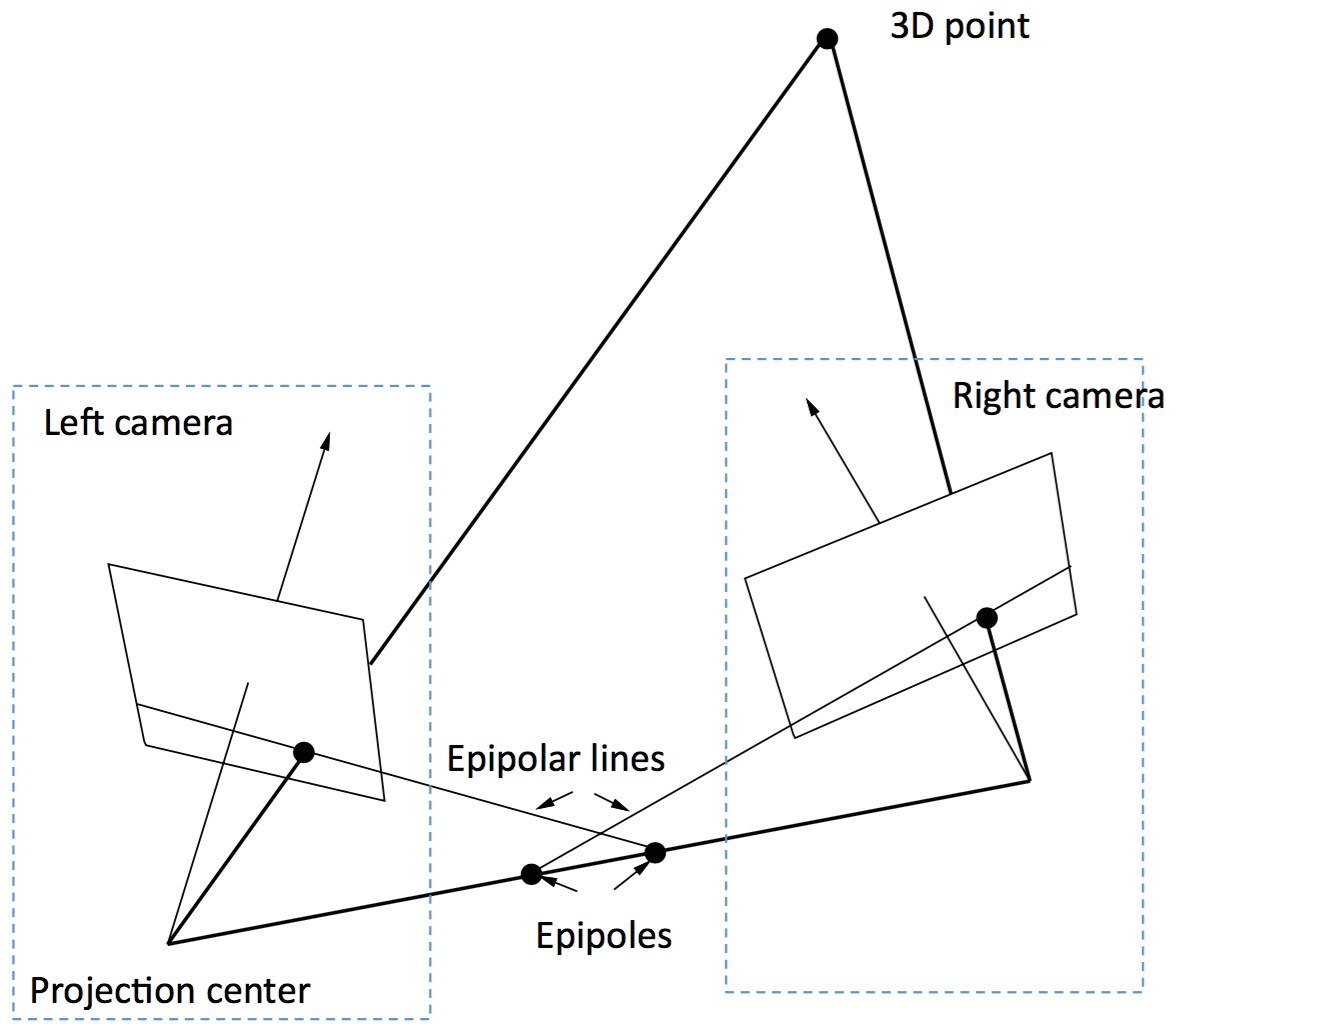
\includegraphics[width=0.40\linewidth]{figures/camera_passive.png}}
\subfigure[Active stereo]{\label{fig:rgbd_camera_active} 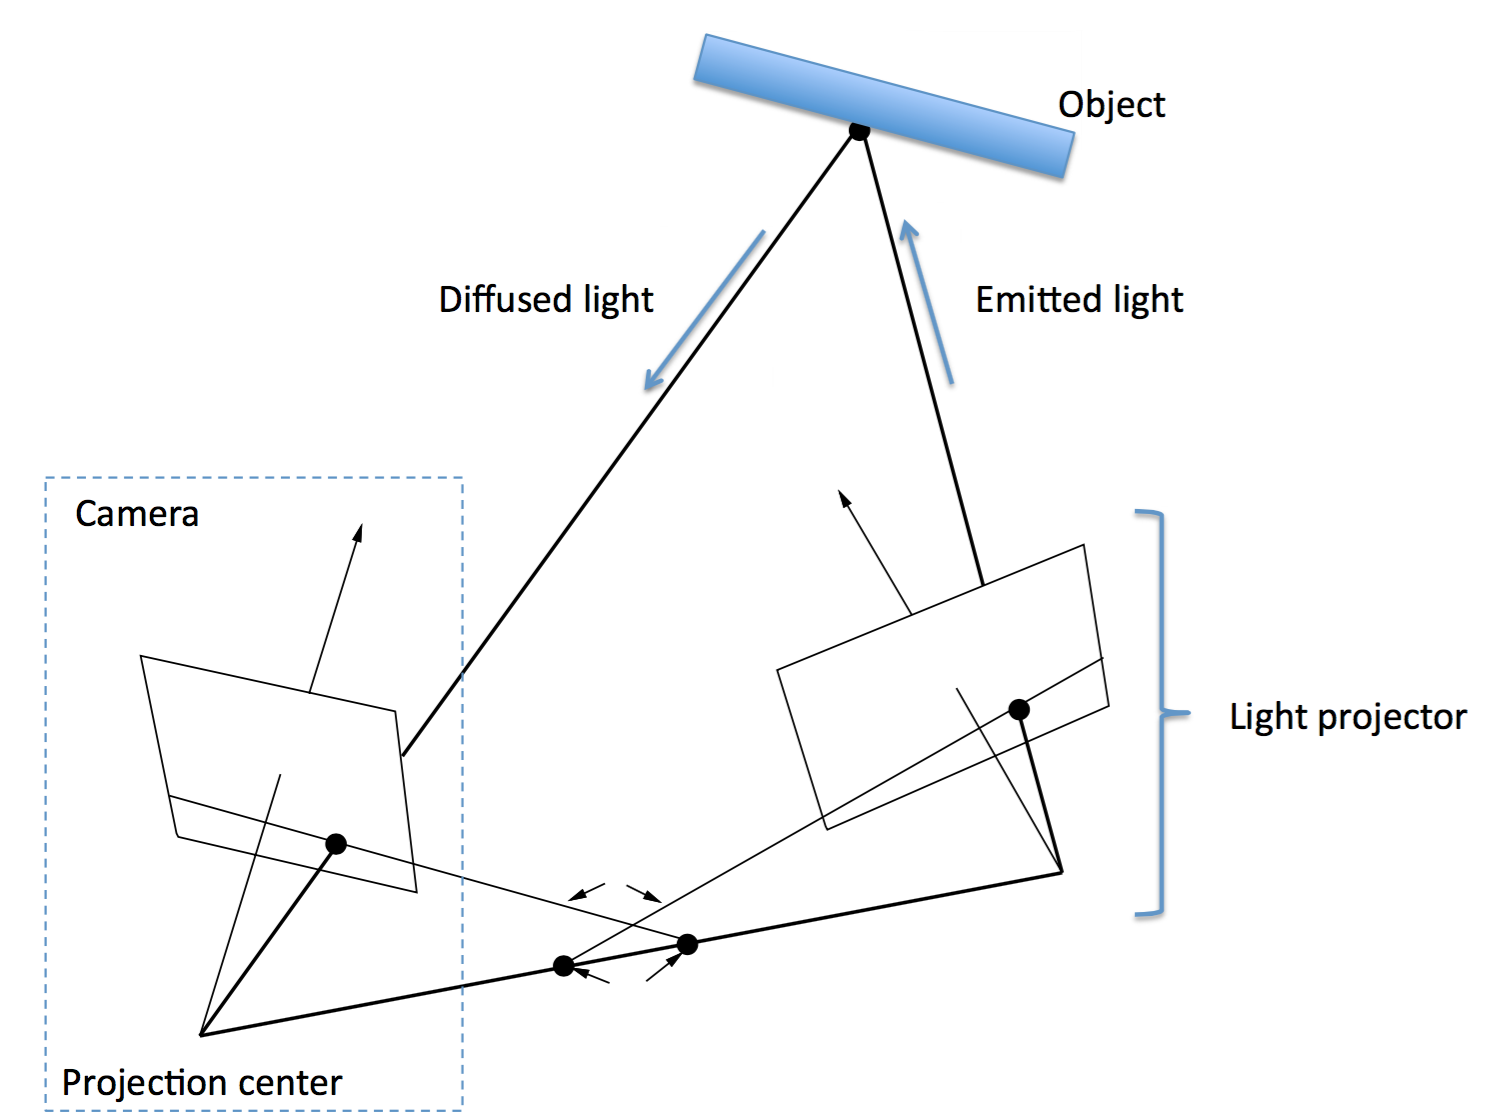
\includegraphics[width=0.45\linewidth]{figures/camera_active.png}}
\caption{Illustrations for the principle of passive and active stereo. Image courtesy of~\cite{horaud2013tutorial}.}
\label{fig:rgbd_camera}
\end{figure}


%%%%%%%%%%%%%%%%%%%%%%%%%%%%%%%%%%%%%%%%%%%%
\subsection{ASUS Xtion PRO LIVE}
%%%%%%%%%%%%%%%%%%%%%%%%%%%%%%%%%%%%%%%%%%%%

\begin{figure}[!ht]
\centering
\subfigure[Camera structure~\cite{asus}]{\label{fig:asus_structure} 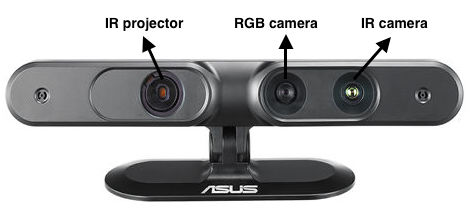
\includegraphics[width=0.4\linewidth]{figures/asus.jpg}}\\
\subfigure[RGB image]{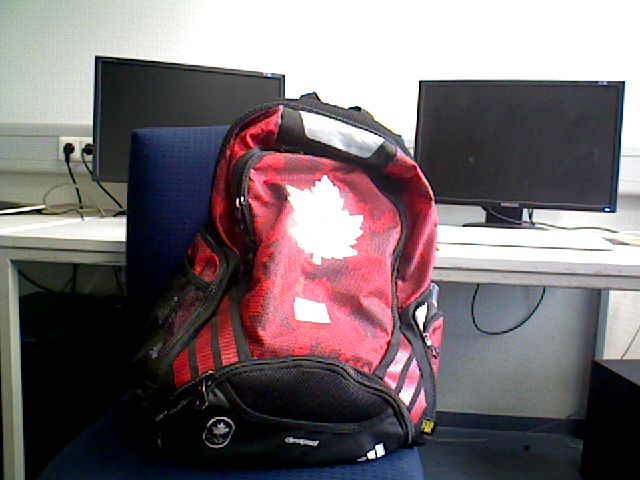
\includegraphics[width=0.4\linewidth]{figures/scene_rgb.png}}
\subfigure[Depth image]{ 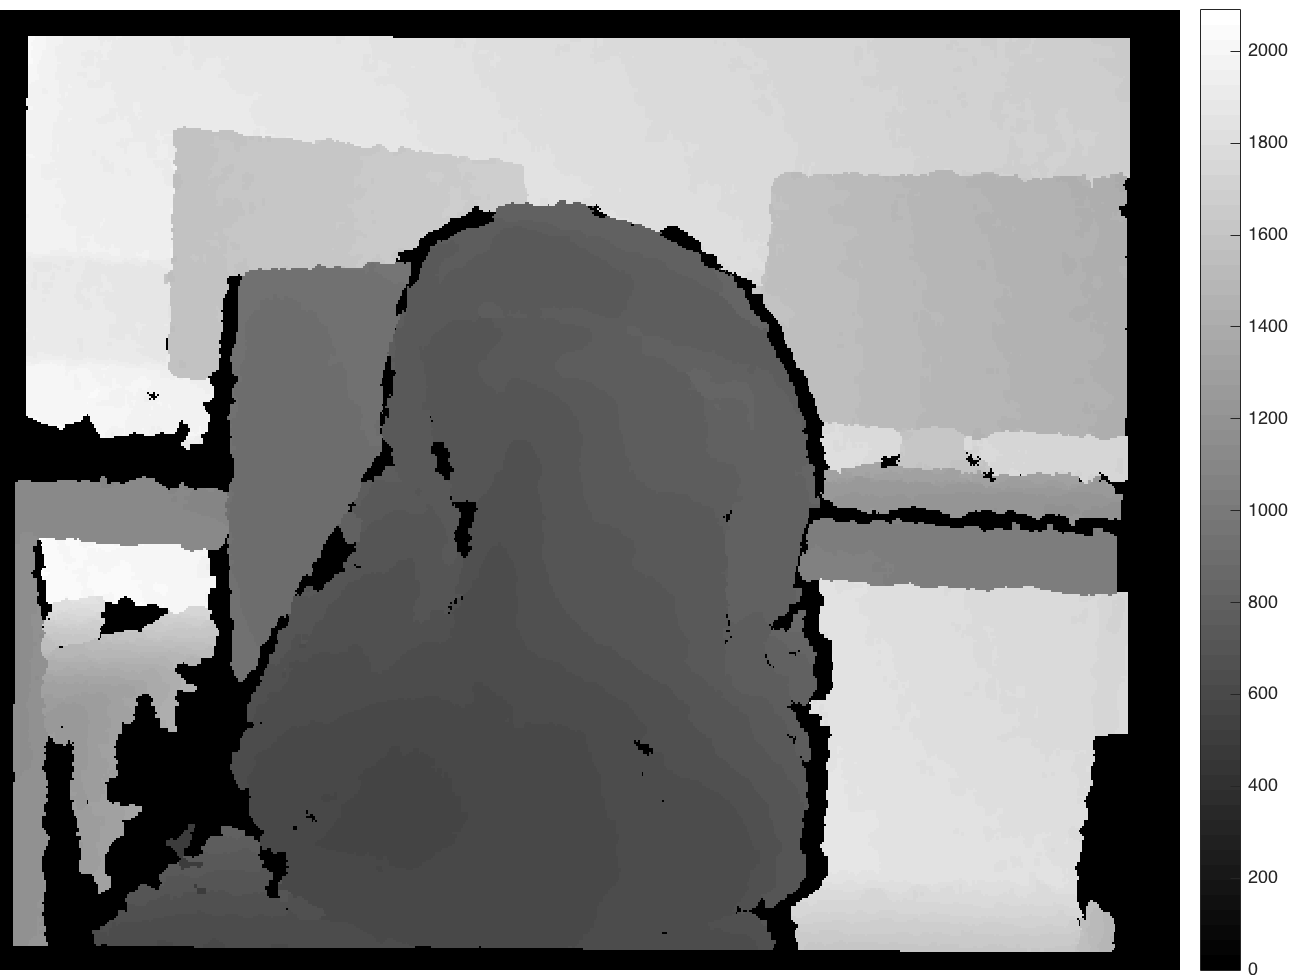
\includegraphics[width=0.4\linewidth]{figures/scene_depth.png}}
\caption{The structure of ASUS Xtion Pro Live and the RGB and depth images of an indoor scene acquired by it.}
\label{fig:asus_illustration}
\end{figure}
The ASUS Xtion Pro Live camera has two cameras and a projector as shown in Fig.~\ref{fig:asus_structure}.
Based on the official website, it provides the RGB image with the maximum resolution of $1280\times1024$, and the depth can be alternated either VGA resolution ($640\times480$ with 30fps) or QVGA ($320\times240$ with 60fps). 
Its depth ranges from 0.8 to 3.5m, but we found in the experiments that the blind area was around 0.5m.  
Xtion Pro Live has been used throughout our experiments.
When the depth super-resolution is required, the RGB images have the resolution of $1280\times1024$, otherwise we keep the same resolution as the depth ($640\times480$).
Based on our applications, we choose different configurations. mentioned our applications.

%%%%%%%%%%%%%%%%%%%%%%%%%%%%%%%%%%%%%%%%%%%%
\section{Shape from Shading \& Photometric Stereo}

\begin{enumerate}
\item First several sentences about SFS, first formularized by  Horn~\cite{horn1970shape}, it can solve simple inputs but not the complicated ones, show one image about its local ambiguity

\item then give the definition of Lambertian reflectance model (first derive the model like intrinsic image decomposition, show an image here), then expend to light * albedo * normal, which is first introduced by Hayahawa 94. 

\item then naturally comes to the definition of normal (orthographic and the perspective)

\item then to solve the Lambertian model to get the 2 DOF gradients, some constraints are imposed on the filed of surface normals. The integrability constraint is imposed by many people ($p_y = q_x$) to make the problem well-posed like Horn and Brooks~\cite{horn1986variational},  {\color{red}Frankot and Chellapa~\cite{frankot1988method} use orthogonal projection to the subspace of valid smooth surfaces}, some people use curl operator to impost this constraint~\cite{han2013high}.

\item then calibrated PS . Give an matrix form like $I = BS$ ({\color{red} or should we?}), B ecodes the surface normal times the albedo. Woodham comes in and there is no need to impose the intergrability constraint but using several images from different directions, and since the lights $S$ are known, a LS is used for such a over-constrined system. Forsythe and Ponce takes care of the pixels which values are zero.

\item However, the lighting $S$ is not always known so the uncalibrated photometric stereo comes to the stage. Hayahawa 94 find that the surface normals ans the albedo can be recovered with a $3\times3$ linear transformation using SVD. Yuille 97 adding the integrabiilty constraint reduced the number of ambiguities to 3 parameters, which we call Gerneralized Bas-Relief (GBR). (Here we should put an image illustrating the ambiguities of shape)

\item Talk about several methods to solve this ambiguity (We can refer to Queau's 2015 paper to put related methods about resolving the GBR ambiguity)

\item Then we say since the rough depth is given as the input, such ambiguity is not a problem anymore , so we move to next subsection: depth refinement.

\end{enumerate}

{\color{red} Questions:}
\begin{enumerate}
\item Where to put the "perspective projection" and second order SH? It seems it will become less continuous if we put them right after the orthographic projection and the Lambertian. Maybe put in the depth refinement? 
\item where to put Hernandez PAMI paper? Their goal was to overcome the shadows but it seems that we didn't really follow theirs
\end{enumerate}

Shape from Shading (SFS) uses a single image to estimate the surface using knowledge of the light source position, albedo and position of the camera. The integrability constraint is imposed as a constraint in optimization to make the problem well posed, as described by Horn and Brooks~\cite{horn1986variational}.
The reason why the integrability constraint is applied is that surface normal will not be an arbitrary vector field
They used an iterative variational scheme to solve for the first order partial derivative of the depth, not strictly enforcing the integrability constraint, but using it as a penalty in the minimization function.
 Frankot and Chellapa~\cite{frankot1988method} use orthogonal projection to the subspace of valid smooth surfaces at each iteration of the Horn and Brooks algorithm. (Here we can introduce orthogonal projection model, we assume that the image plane is directly above the surface)
 
In Photometric stereo (PMS), the integrability constraint is not used at all. At least three images are taken of the object with known (or estimated) light sources.  In the basic algorithm, the surface normals are estimated using Least-Square solution (Woodham 1980~\cite{woodham1980photometric}), and no global information is used at all in the estimation. 

The whole paragraph above was from~\cite{petrovic2001enforcing}






%%%%%%%%%%%%%%%%%%%%%%%%%%%%%%%%%%%%%%%%%%%%
there exist infinite solutions if only the SFS term is applied to refine the depth (Yvain's PhD thesis). Therefore, z-z0 data fidelity is albedo to applied to restrict to the unique solution 
%----------------------------------------------
\subsection{Lambertian reflectance model}
%----------------------------------------------
We can show the Intrinsic image decomposition as the an example of Lambertian reflectance as an informal explanation. shading is the product of the a certain kind of illumination model and the shape (surface normal)~\cite{barron2015shape}

Illustrate with the an image from MIT intrinsic dataset~\cite{grosse2009ground}

SH model is an extension of Lambertian model

  \url{https://pdfs.semanticscholar.org/7b8d/fc5d6e276f8048bb53b4a5e0611019570f1b.pdf}
\cite{basri2003lambertian}

cite Shape From Shading Emmanuel Prados, Olivier Faugeras
\url{https://en.wikipedia.org/wiki/Lambertian_reflectance}

\url{https://www.cs.cmu.edu/afs/cs/academic/class/15462-f09/www/lec/lec8.pdf}
\url{http://www.cs.virginia.edu/~gfx/Courses/2011/ComputerVision/slides/lecture20_pstereo.pdf}


we assume that surfaces in a scene are Lambertian, and we parameterize the incident lighting with spherical harmonics (SH) [Wu et al. 2011] \cite{wu2011shading}.

In fact, we estimate incident irradiance as a function of the surface normal, that is the incident light, filtered by the cosine with the normal. For Lambertian reflectance, the incident irradiance function is known to be smooth, and can be represented with only little error using the first nine spherical harmonics basis functions up to 2nd order~\cite{ramamoorthi2001efficient}. (well, actually should check this one~\cite{ramamoorthi2001relationship})
As with previous approaches, we henceforth estimate lighting from a grayscale version of I, and thus assume gray lighting with equal values in each RGB channel. In some steps, full RGB images are used, which we denote Ic. Unlike offline multi-view methods, we employ a triangulated depth map as geometry parameterization. This means there is a fixed depth pixel to mesh vertex relation, and we can express the reflected irradiance B(i, j) of a depth pixel (i, j) with normal n(i, j) and albedo k(i, j)

This sentence is from\cite{wu2014real}


%----------------------------------------------
\subsection{Surface normal}
%----------------------------------------------
\url{http://docs.opencv.org/2.4/modules/calib3d/doc/camera_calibration_and_3d_reconstruction.html}

orthographic model
perspective model

It is an ill-posed problem to estimate the normal, that's where SFS and PS are involved. 

SFS:
Horn

PS:

calibrated light: woodham~\cite{woodham1980photometric} \url{https://classes.soe.ucsc.edu/cmps290b/Fall05/readings/Woodham80c.pdf}

uncalibrated light:

Hayakawa 94~\cite{hayakawa1994photometric} \url{http://www.wisdom.weizmann.ac.il/~vision/courses/2010_2/papers/photometric_stereo.pdf}
start the I = albedo*light*normal $3\times3$ linear ambiguity

Yville 97~\cite{yuille1997shape}: \url{http://citeseerx.ist.psu.edu/viewdoc/download?doi=10.1.1.446.3648&rep=rep1&type=pdf}
use integrability (smoothness), reduce the ambiguity to 3-parameter ambiguity (GBR)
$z(x,y) = \lambda z(x,y) + \mu x + \beta y$, which is GBR ambiguity. That's why our method works because we have initial depth $z_0$ and data fidelity term constrains the $z$ to $z_0$, so the ambiguity equation is invalid. 
And in our case: PDE ($\Delta z$) $->$ integrability is implicity enforced

All the following PS method is trying to solve this ambiguity
alldrin 07~\cite{alldrin2007resolving} use entropy \url{http://citeseerx.ist.psu.edu/viewdoc/download?doi=10.1.1.93.7264&rep=rep1&type=pdf}

\cite{papadhimitri2013new} perspective \url{http://www.cv-foundation.org/openaccess/content_cvpr_2013/papers/Papadhimitri_A_New_Perspective_2013_CVPR_paper.pdf}

\cite{papadhimitri2014closed}\url{https://pdfs.semanticscholar.org/2cf9/088e9faa81872b355a4ea0a9fae46d3c8a08.pdf}

\cite{queau2015solving} use TV \url{http://oatao.univ-toulouse.fr/15158/1/queau_15158.pdf}


%%%%%%%%%%%%%%%%%%%%%%%%%%%%%%%%%%%%%%%%%%%%
%\section{Intrinsic Image Decomposition}
%%%%%%%%%%%%%%%%%%%%%%%%%%%%%%%%%%%%%%%%%%%%

\section{Depth Map Refinement}
%%%%%%%%%%%%%%%%%%%%%%%%%%%%%%%%%%%%%%%%%%%%

My feeling: the state-of-the-art depth refinement method using single image is just an extension of SFS (not even PS), but instead of estimating the two surface gradients from the intensity, they are only interested in the one depth, and the problem becomes even easier because of the input rough depth.

The depth refinement can be divided to two categories: SFS based method and the PS based method.

Since SFS iteslf uses only one input image, it suffers from some intrinsic ambiguities that we have mentioned in the last section even when the lights is known, so there will be more than one possible solutions.
Moreover, SFS methods are often limited to the uniform or constant albedo. 
Some methods~\cite{han2013high, yu2013shading} adapted segmentation methods to divide the input image into some constant albedo part, but the real-world objects are usually with complex multi-albedo and small regions, which makes the segmentation not accurate or incorrect.  
Therefore, SFS methods using only one single image have the difficulty to separate the albedo from the surface normal, which leads to the wrong depth estimation.

Han \emph{et al.}~\cite{han2013high} presented a framework which combines a global lighting model using the given color and depth with the help of SH model, with a local lighting model which varies spatially. 
The surface orientations should obey the integrability constraint on the smooth surface so they enforced the constraint by penalizing the curl of local neighborings.
However, the albedo in their method is assumed to be uniform.
To handle the multi-albedo objects, they had to apply another intrinsic image decomposition algorithm~\cite{barron2011high} and k-mean clustering to group the albedos.
Such framework is very time-consuming and not able to be adapted to the real-world applications.

Yu \emph{et al.}~\cite{yu2013shading} iteratively update SH lighting and the albedo using the initial depth and the refined the shape with the estimated lighting and the relative albedo. 
They performed mean-shift clustering to segment the input RGB image into small regions with uniform albedo, and then obtained the relative albedos among various segmented regions. 
To fill in the missing depth information, a constrained texture synthesis and patch-based repairing scheme was applied.
In constrast, we efficiently apply an basic image inpainting approach as the pre-processing and the results are also satisfying.


Wu \emph{et al.}~\cite{wu2014real} extended their previous offline shading-based refinement work~\cite{wu2011shading} with highly parallel scheme and the help of GPU. 
They first calculated the 2nd-order SH parameters with the assumption of uniform albedo, and then estimated the albedo by simply dividing RGB image with the shading term.
We discuss in chapter~\ref{chap:methodology} that severe overfitting problem will happen with this process such that the albedo estimation is not correct.
The shape is then refined in real-time by finding the surface that minimizes the difference between the shading and intensity image gradients.
Thereafter, the coarse depth map was directly refined with smoothness and temporal constraint on the video by using a Gauss-Newton solver on GPU.

Kim \emph{et al.}~\cite{kim2015joint} used a joint energy to estimate the depth, albedo and the light with smoothness regularization terms.
An anisotropic Laplacian constraint on chromaticity was introduced for albedo and a local smoothness and bas-relief ambiguity similar to~\cite{barron2013intrinsic} constraints are imposed for depth.
Based on our experiments, it has turned out that the Laplacian on chromaticity of the image cannot provide satisfying albedos inside the small indoor environment.
What's more, it is a very tedious process to tune all the parameters for the constraints.

Or-El's 2016 paper~\cite{or2016real} can deal with specular objects with the help of IR camera and a more complicated model than SH. 
Instead, our method still uses a Lambertian diffused reflectance model but can handle the specularity because the specular parts inside the image.


Depth refinement with PS: With the help of multiple images acquired from various illuminations, PS based depth refinement methods can resolve the ambiguities tolerated by SFS methods 

Haque \emph{et al.}~\cite{haque2014high} was the first method to reconstruct the shape and refine the depth using an IR camera without the need of RGB camera.
However, the problem is the same as many other multi-view photometric reconstruction approaches~\cite{park2013multiview, queau2017dense} that the albedo is restricted to uniform.

Their follow-up work from Chatterjee and Govindu~\cite{chatterjee2015photometric} decomposed the input images under different illuminations with a standard photometric stereo manner.
They used an iterative reweighted method to approximate the Rank 3 radiometric brightness matrix, then factorize it into the corresponding lighting, albedo and surface normal. 
They can cope with the multi-albedo objects but still have to use the IR images instead of RGB images. 
In this case, an extra infrared light source is required, while in our case only a cheap LED light or even just the flashlight on a phone is enough.
Moreover, since the IR camera in ASUS Xtion Pro Live is limited to the resolution $640\times 480$, while the RGB camera can reach $1280\times 1024$, the depth super-resolution task can be performed with our method.

mention Super-resolution Imaging that it is also very interesting to extend our the state-of-the-art depth refinement to real refinement.



Multi-view-stereo 
Wu~\cite{wu2011high} uses a second-order spherical harmonics to model the general illuminations and use the shading constraint to help improve the object reconstruction.
this method is extended to~\cite{wu2011shading} whose results are furthered improved by integrating a weak temporal prior on lighting, albedo and the shape.
mentioned very latest research is also related to depth refinement, using several images from different views (Yvain's and Zuozuo's Arxiv paper) 
%%%%%%%%%%%%%%%%%%%%%%%%%%%%%%%%%%%%%%%%%%%%

%
%\begin{figure}[htb]
%        \centering
%        \epsfxsize=4cm
%        {\epsfbox{figures/interp.eps}}
%  \caption{Interpolation of corresponding coordinates}
%  \label{fig:interp}
%\end{figure}
%
